\title{Kepler's Laws of Planetary Motion}
\author{Dr. Jordan Hanson - Whittier College Dept. of Physics and Astronomy}
\date{\today}
\documentclass[12pt]{article}
\usepackage[margin=1.25cm]{geometry}
\usepackage{hyperref}
\usepackage{graphicx}
\usepackage{amsmath}
\usepackage{subcaption}
\begin{document}
\maketitle

\small

\begin{figure}[ht]
\centering
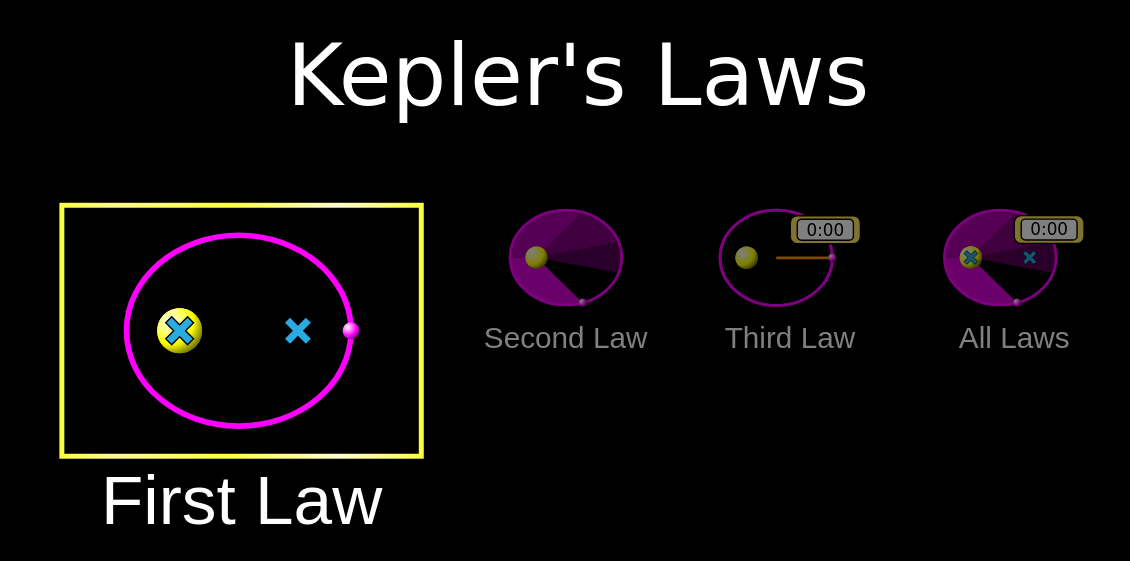
\includegraphics[width=0.33\textwidth]{figures/kepler3.png}
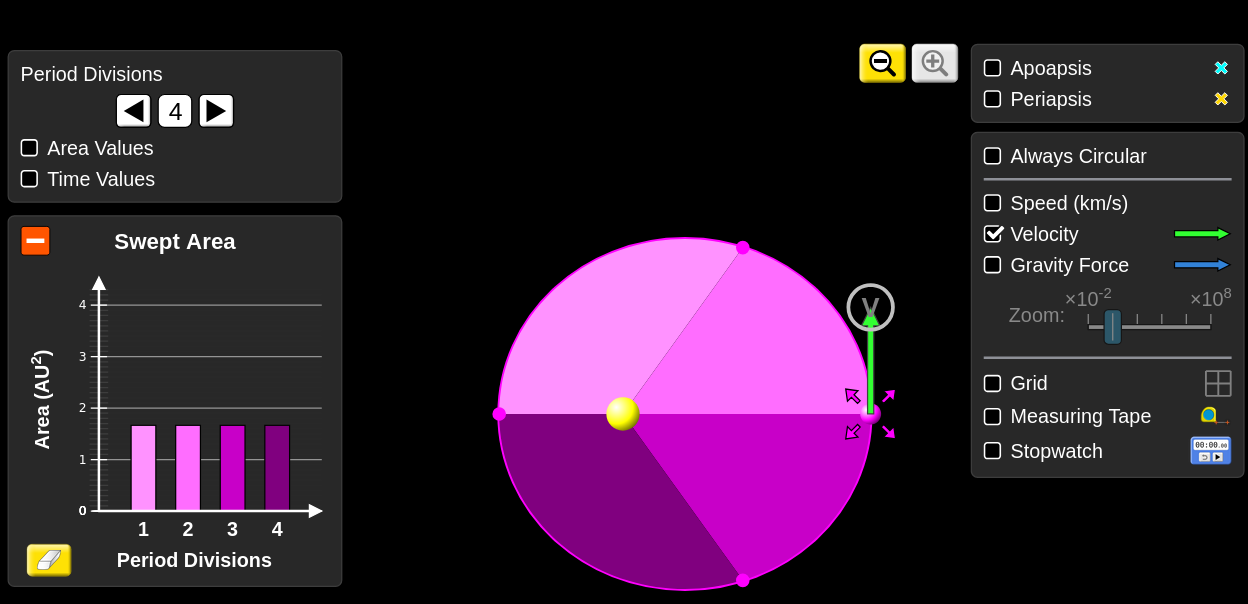
\includegraphics[width=0.34\textwidth]{figures/kepler2.png}
\caption{\label{fig:1b} A PhET simulation exploring Kepler's Laws}
\end{figure}

\section{Introduction}

When reading \textit{Science in Latin America}, we encounter references to the debate between a heliocentric universe and a geocentric universe.  To understand this debate within Latin American scientific circles, we will explore Kepler's Laws using the following simulation: \url{https://phet.colorado.edu/en/simulations/keplers-laws}.

\section{Kepler's First Law}

\textit{The orbit of a planet is an ellipse with the Sun at one of the two foci.}  (a) Open the First Law tab in the simulation.  Using the controls, set the target orbit to Venus.  (b) Arrange the velocity and position of the planet so that the orbit matches that of Venus. Click the play button.  (c) Now set the target orbit to that of the Earth.  (d) Why are we (rarely) able to observe Venus transit across the face of the Sun, from our perspective? \\ \vspace{0.25cm}

\section{Kepler's Second Law}

\textit{A line segment joining a planet and the Sun sweeps out equal areas during equal intervals of time.} (a) Open the Second Law tab in the simulation.  Using the controls at the upper left, set the period divisions to 6, and check the area and time boxes.  (b) Activate the orbit and note that the ratio of area to time is constant.  (c) Change the orbital parameters and repeat the measurement.

\section{Kepler's Third Law}

\textit{The square of a planet's orbital period is proportional to the cube of the length of the semi-major axis of its orbit.} (a) \textit{Observe the proof of Kepler's Third Law on the board.}  (a) Now that we have predicted the relationship between \textit{T} and \textit{a}, activate the orbit to obtain \textit{T} and \textit{a} data in the graph of \textit{T} vs. \textit{a} on the left side.  (b) Change the orbit to add more data.  (c) Change the graph to different powers of \textit{T} and \textit{a} until the graph is a straight line with a slope of 1.

\end{document}
